\documentclass[a4paper,11pt]{article}
\input{/home/tof/Documents/Cozy/latex-include/preambule_lua.tex}
\newcommand{\showprof}{show them}  % comment this line if you don't want to see todo environment
\fancyhead[L]{Projet Le morpion}
\newdate{madate}{10}{09}{2020}
\fancyhead[R]{Première - NSI} %\today
\fancyfoot[L]{~\\Christophe Viroulaud}
\fancyfoot[C]{\textbf{Page \thepage}}
\fancyfoot[R]{\includegraphics[width=2cm,align=t]{/home/tof/Documents/Cozy/latex-include/cc.png}}
\usepackage{tikz}

\begin{document}
\begin{Form}
\section{Présentation du projet}
Afin de mettre en application les notions de programmation abordées en cours, nous allons développer le jeu du \emph{morpion}. Le principe est le suivant:
\begin{itemize}
\item Une grille de 3×3 cases.
\item Deux joueurs jouant à tour de rôle.
\item Chaque joueur place un pion (X ou O) sur une case vide.
\item Le gagnant est celui qui aligne trois pions.
\end{itemize}
\medskip
Le projet sera réalisé en groupe de deux. Nous consacrerons quelques temps en classe pour avancer, effectuer des points de vérification, apporter des aides. Cependant il est indispensable de progresser en dehors des heures de cours pour mener le projet à terme. 
\section{Étapes}
\subsection{Contraintes}
Le programme devra:
\begin{itemize}
\item demander les coordonnées de placement du pion en respectant la figure \ref{grille},
\item afficher, dans la console, la grille actualisée à chaque tour de jeu.
\end{itemize}
\begin{figure}[!h]
\centering
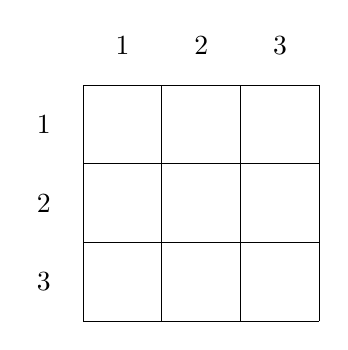
\begin{tikzpicture}
\draw (0,0) grid (3,3);

\draw (-0.5,2.5) node{1};
\draw (-0.5,1.5) node{2};
\draw (-0.5,0.5) node{3};
\draw (0.5,3.5) node{1};
\draw (1.5,3.5) node{2};
\draw (2.5,3.5) node{3};
\end{tikzpicture}
\captionof{figure}{Système de coordonnées}
\label{grille}
\end{figure}

\subsection{Découpage}
Le premier point consiste à réfléchir aux différentes étapes du déroulement du jeu. Il peut être utile ici de noter les idées sur papier afin de pouvoir présenter et retravailler ce séquençage avec l'enseignant.
\subsection{Notions nécessaires}
Les \emph{constructions élémentaires de programmation} abordées en classe sont suffisantes pour réaliser ce projet. Bien sûr il sera possible d'introduire des notions vues ultérieurement ou découvertes grâce à des recherches personnelles.
\section{Évaluation}
L'évaluation comportera trois axes:
\begin{itemize}
\item le respect des principes du jeu,
\item le partage des tâches dans le groupe,
\item la clarté du code (commentaires, espace, constructions optimisées)
\end{itemize}
\end{Form}
\end{document}